% =====================================================================
%  MiniVPN -- Computer Networks Lab Synopsis
%  Compile:  pdflatex cn-synopsis.tex   (run twice for references)
%  Needs jiit-logo.png in the same folder.
% =====================================================================
\documentclass[12pt,a4paper]{article}

\usepackage[margin=1in]{geometry}
\usepackage{graphicx}
\usepackage{setspace}
\usepackage{enumitem}
\usepackage{booktabs}
\usepackage{tabularx}
\usepackage{xcolor}
\usepackage{tikz}
\usetikzlibrary{positioning,arrows.meta,shapes.geometric,fit}
\usepackage[hidelinks]{hyperref}

\setstretch{1.25}
\setlist{itemsep=2pt,topsep=4pt}

% Running header and page number (no extra package needed)
\makeatletter
\def\ps@project{%
  \def\@oddhead{\small MiniVPN -- CN Lab Synopsis\hfill JIIT, Noida}%
  \let\@evenhead\@oddhead
  \def\@oddfoot{\hfil\thepage\hfil}%
  \let\@evenfoot\@oddfoot}
\makeatother
\pagestyle{project}

% ---------------------------------------------------------------------
%  Front-page details -- edit here
% ---------------------------------------------------------------------
\newcommand{\projecttitle}{MiniVPN: Design and Implementation of a Secure Layer-3 Tunnelling Protocol over UDP}
\newcommand{\doctype}{Computer Networks Lab Synopsis}
\newcommand{\semester}{Semester 5}

\begin{document}

% =========================== FRONT PAGE ==============================
\begin{titlepage}
\centering
{\Large\bfseries BACHELOR OF TECHNOLOGY\par}
\vspace{1.2cm}

\includegraphics[width=4.2cm]{jiit-logo.png}\par
\vspace{0.6cm}
{\large Jaypee Institute of Information Technology, Noida\par}
\vspace{1.4cm}
{\LARGE\bfseries \projecttitle\par}
\vspace{1.2cm}
{\Large \semester\par}
\vspace{0.4cm}
{\Large\bfseries \doctype\par}
\vfill
\begin{minipage}[t]{0.52\textwidth}
\raggedright
{\large\bfseries Made By:}\\[6pt]
Sansriti Mishra \hfill 2401030293\\
Mokshi Mittal \hfill 2401030326\\
Sanvi Dhingra \hfill 2401030312
\end{minipage}%
\hfill
\begin{minipage}[t]{0.38\textwidth}
\raggedleft
{\large\bfseries Submitted To:}\\[6pt]
Dr. Anuja Shukla\\
Dr. Kirti Agarwal
\end{minipage}
\vspace{1.5cm}

{\large Department of Computer Science \& Engineering and IT\par}
\end{titlepage}

% ============================ BODY ===================================

\section{Introduction}
A \emph{Virtual Private Network} (VPN) builds a private network on top of a public one.
IP packets travelling between members of the VPN are \emph{encapsulated} inside other
packets, encrypted and authenticated, then carried across the Internet. To the
applications at either end, remote machines appear to be on the same local subnet.

\textbf{MiniVPN} is a layer-3 VPN written from scratch in C. It carries IPv4 packets
inside UDP datagrams, using its own binary wire protocol, handshake and reliability
mechanisms. The project lets us apply the core topics of computer networks directly:
the TCP/IP layering model, IPv4 addressing and subnetting, routing and longest-prefix
match, MTU and fragmentation, NAT, transport over UDP, and secure protocol design.

\section{Problem Statement}
Organisations need to connect remote laptops, servers and branch offices into one
private network across the untrusted Internet. The solution must:
\begin{itemize}
  \item carry arbitrary IP traffic (ping, SSH, HTTP) between devices transparently;
  \item keep that traffic confidential and tamper-proof on the public network;
  \item work through home routers and mobile networks that use NAT, and survive a device
        changing its network (Wi-Fi to mobile data);
  \item recover from packet loss, since UDP itself gives no delivery guarantee;
  \item let an administrator add or revoke devices while the network is running.
\end{itemize}

\section{Objectives}
\begin{enumerate}
  \item Design an \textbf{IP-in-UDP encapsulation} protocol with a compact, byte-level packet format.
  \item Implement a \textbf{one-round-trip authenticated handshake} that establishes fresh
        session keys (X25519 key exchange, HKDF, HMAC).
  \item Protect data with \textbf{authenticated encryption} (ChaCha20-Poly1305), an
        \textbf{anti-replay window} and \textbf{source-address anti-spoofing}.
  \item Assign each device a fixed address from a \textbf{tunnel subnet} (10.8.0.0/24) and route
        packets between devices and to the Internet through \textbf{NAT}.
  \item Handle \textbf{MTU} correctly so tunnelled packets do not fragment on a 1500-byte path.
  \item Add \textbf{reliability over UDP}: retransmission with exponential backoff, keepalives,
        dead-peer detection, NAT traversal and roaming.
  \item Support a \textbf{full-tunnel} mode that redirects all traffic using longest-prefix routing.
  \item Verify behaviour with packet captures and end-to-end tests across isolated virtual networks.
\end{enumerate}

\section{Proposed System Architecture}

\begin{figure}[h]
\centering
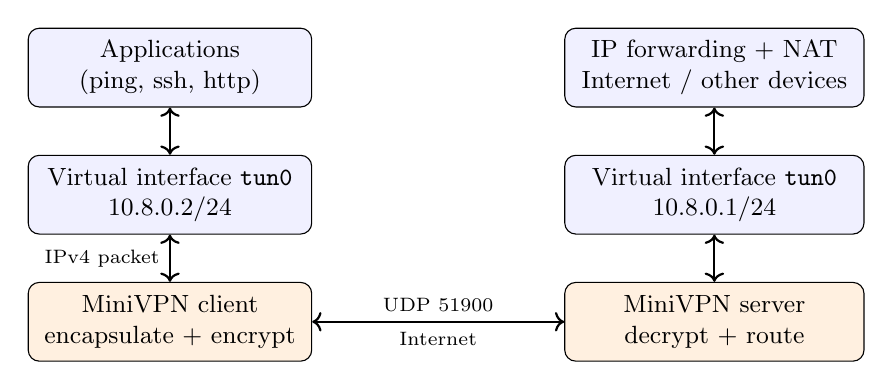
\begin{tikzpicture}[
  box/.style={draw,rounded corners,align=center,minimum height=1cm,font=\small,fill=blue!6},
  arr/.style={-{Stealth},thick}]
  \node[box,minimum width=3.6cm] (app) {Applications\\(ping, ssh, http)};
  \node[box,below=0.6cm of app,minimum width=3.6cm] (tun) {Virtual interface \texttt{tun0}\\10.8.0.2/24};
  \node[box,below=0.6cm of tun,minimum width=3.6cm,fill=orange!12] (cli) {MiniVPN client\\encapsulate + encrypt};
  \node[box,right=3.2cm of cli,minimum width=3.8cm,fill=orange!12] (srv) {MiniVPN server\\decrypt + route};
  \node[box,above=0.6cm of srv,minimum width=3.8cm] (stun) {Virtual interface \texttt{tun0}\\10.8.0.1/24};
  \node[box,above=0.6cm of stun,minimum width=3.8cm] (lan) {IP forwarding + NAT\\Internet / other devices};
  \draw[arr,<->] (app) -- (tun);
  \draw[arr,<->] (tun) -- node[left,font=\scriptsize]{IPv4 packet} (cli);
  \draw[arr,<->] (cli) -- node[above,font=\scriptsize]{UDP 51900}
                          node[below,font=\scriptsize]{Internet} (srv);
  \draw[arr,<->] (srv) -- (stun);
  \draw[arr,<->] (stun) -- (lan);
\end{tikzpicture}
\caption{High-level architecture of MiniVPN}
\end{figure}

\begin{figure}[h]
\centering
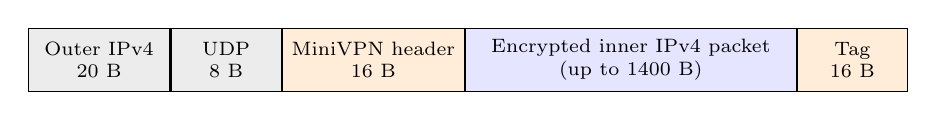
\begin{tikzpicture}[f/.style={draw,minimum height=0.8cm,font=\scriptsize,align=center}]
  \node[f,fill=gray!15,minimum width=1.8cm] (a) {Outer IPv4\\20 B};
  \node[f,fill=gray!15,minimum width=1.4cm,right=0pt of a] (b) {UDP\\8 B};
  \node[f,fill=orange!15,minimum width=2.2cm,right=0pt of b] (c) {MiniVPN header\\16 B};
  \node[f,fill=blue!10,minimum width=4.2cm,right=0pt of c] (d) {Encrypted inner IPv4 packet\\(up to 1400 B)};
  \node[f,fill=orange!15,minimum width=1.4cm,right=0pt of d] (e) {Tag\\16 B};
\end{tikzpicture}
\caption{Encapsulation of a tunnelled packet}
\end{figure}

An application sends an ordinary IP packet. The kernel routes it to the virtual
interface \texttt{tun0}, from which the MiniVPN client reads it. The client encrypts it,
adds a 16-byte header and a 16-byte authentication tag, and sends the result as a UDP
datagram to the server. The server verifies and decrypts it, checks that the inner
source address belongs to that device, and either forwards it to another device or
hands it to the kernel, which routes it onward (through NAT for Internet traffic).

\section{Networking Concepts Applied}
\begin{tabularx}{\textwidth}{@{}lX@{}}
\toprule
\textbf{Concept} & \textbf{Use in MiniVPN}\\
\midrule
Layering \& encapsulation & IP packet carried as the payload of a UDP datagram (IP-in-UDP)\\
IPv4 header & Version, total length, source and destination addresses parsed for routing and anti-spoofing\\
Addressing \& subnetting & Tunnel subnet 10.8.0.0/24; server .1, devices get fixed host addresses\\
Routing & Server routes by destination IP; full tunnel uses \texttt{0.0.0.0/1} + \texttt{128.0.0.0/1} (longest-prefix match) with a pinned /32 host route to the server\\
MTU \& fragmentation & 60 bytes of overhead; tunnel MTU 1400 so packets fit a 1500-byte path with DF set\\
NAT & Server masquerades the VPN subnet to the Internet; keepalives hold client-side NAT mappings open\\
Transport (UDP) & Connectionless transport; reliability for the handshake added on top\\
Reliability & Retransmission with exponential backoff, keepalives, timeouts, dead-peer detection\\
Mobility & Roaming: session follows the client's new IP:port after authenticated packets\\
Network security & Authenticated key exchange, AEAD, replay window, forward secrecy\\
Application layer & HTTP web dashboard with cookies, CSRF protection and optional TLS\\
\bottomrule
\end{tabularx}

\section{Methodology}
\begin{enumerate}
  \item \textbf{Tunnel layer:} create a TUN virtual interface that exchanges raw IPv4 packets
        with the kernel; build a plaintext IP-in-UDP tunnel between two hosts.
  \item \textbf{Protocol design:} define HELLO, WELCOME, DATA, KEEPALIVE and DISCONNECT messages
        with fixed, big-endian (network byte order) field layouts.
  \item \textbf{Security:} authenticated handshake, per-direction session keys, AEAD data channel,
        1024-packet replay window.
  \item \textbf{Routing:} per-device address assignment, server-side forwarding between devices,
        NAT for Internet access, optional full-tunnel routing on the client.
  \item \textbf{Robustness:} MTU sizing, retransmission and backoff, keepalives, session timeouts,
        roaming and periodic rekeying.
  \item \textbf{Testing:} build a virtual topology of several hosts with Linux network namespaces
        and \texttt{veth} links; verify with \texttt{ping}, file transfer, \texttt{tcpdump} and Wireshark.
\end{enumerate}

\section{Tools and Technologies}
\begin{tabularx}{\textwidth}{@{}lX@{}}
\toprule
Language & C (C11) for the protocol and daemon; Python 3 for the management dashboard\\
Libraries & OpenSSL \texttt{libcrypto} (X25519, ChaCha20-Poly1305, HMAC-SHA256, Ed25519)\\
Platform & Linux (Ubuntu on WSL2 for development)\\
Network tools & \texttt{ip}, \texttt{ip netns}, \texttt{veth}, \texttt{iptables}, \texttt{tcpdump}, Wireshark, \texttt{ping}\\
Build & GCC, GNU Make\\
\bottomrule
\end{tabularx}

\section{Expected Outcomes}
\begin{itemize}
  \item Devices on different networks communicate over 10.8.0.0/24 as if on one LAN.
  \item Packet captures on the public path show only UDP datagrams with encrypted payloads.
  \item Replayed, modified or spoofed packets are rejected.
  \item Maximum-size packets cross the tunnel without fragmentation.
  \item Connections survive packet loss, NAT and a change of the client's network.
  \item Full-tunnel mode sends all Internet traffic of a device through the VPN server.
\end{itemize}

\section{Work Plan}
\begin{tabularx}{\textwidth}{@{}lX@{}}
\toprule
\textbf{Phase} & \textbf{Activity}\\
\midrule
Week 1--2 & Study tunnelling, TUN interfaces and IP-in-UDP; build a plaintext tunnel between two namespaces\\
Week 3--4 & Packet format, handshake and encrypted data channel; anti-replay window\\
Week 5--6 & Multi-device server, address assignment, routing between devices, NAT\\
Week 7--8 & MTU handling, keepalives, retransmission, roaming, full-tunnel routing\\
Week 9--10 & Testing with packet captures, performance measurement, documentation\\
\bottomrule
\end{tabularx}

\section*{References}
\begin{enumerate}[label={[\arabic*]}]
  \item A. S. Tanenbaum, D. J. Wetherall, \emph{Computer Networks}, 5th ed., Pearson, 2011.
  \item J. F. Kurose, K. W. Ross, \emph{Computer Networking: A Top-Down Approach}, 8th ed., Pearson, 2021.
  \item J. Postel, \emph{Internet Protocol}, RFC 791, 1981; \emph{User Datagram Protocol}, RFC 768, 1980.
  \item J. A. Donenfeld, ``WireGuard: Next Generation Kernel Network Tunnel,'' NDSS, 2017.
  \item P. Srisuresh, K. Egevang, \emph{Traditional IP Network Address Translator}, RFC 3022, 2001.
  \item Y. Nir, A. Langley, \emph{ChaCha20 and Poly1305 for IETF Protocols}, RFC 8439, 2018.
  \item S. Kent, \emph{IP Encapsulating Security Payload (ESP)}, RFC 4303, 2005.
\end{enumerate}

\end{document}
